\documentclass[12pt]{article}

\usepackage{sbc-template}
\usepackage{graphicx,url}
\usepackage[utf8]{inputenc}

\usepackage{wrapfig}
\usepackage{verbatim}
\usepackage{xspace}
\newcommand{\FC}       {Freechains\xspace}
\newcommand{\AMT}      {\emph{AM-Tools}\xspace}
\newcommand{\reps}     {\emph{reps}\xspace}
\newcommand{\onerep}   {\emph{1~rep}\xspace}
\newcommand{\nreps}[1] {\emph{#1~reps\xspace}}
\newcommand{\code}[1]  {\texttt{\footnotesize{#1}}}
\newcommand{\Xon} {$1{\rightarrow}N$\xspace}
\newcommand{\Xno} {$1{\leftarrow}N$\xspace}
\newcommand{\Xnn} {$N{\leftrightarrow}N$\xspace}
\newcommand{\Xoo} {$1{\leftrightarrow}1$\xspace}
\newcommand{\Xo}  {$1{\hookleftarrow}$\xspace}


\newcommand{\amrw}       {\code{AM-rw}\xspace}
\newcommand{\amdiff}     {\code{AM-diff}\xspace}
\newcommand{\ampatch}    {\code{AM-patch}\xspace}
\newcommand{\amcheckout} {\code{AM-checkout}\xspace}
\newcommand{\amcommit}   {\code{AM-commit}\xspace}

\renewcommand{\theenumi}{\alph{enumi}}

\hyphenation{off-line}

\sloppy

\title{
    \AMT: Operating Permissionless JSON Datasets
}

\author{Anonymous}
\address{Anonymous}

\begin{document}

\begin{comment}
- 8 paginas
- Descrição e motivação do problema resolvido pela ferramenta;
- Arquitetura da solução e descrição das principais funcionalidades;
- Descrição da demonstração planejada para o Salão de Ferramentas, informando equipamentos necessários para tal;
- URL onde a ferramenta está disponível (obrigatório na modalidade Código Aberto);
- URL dos manuais e documentação da ferramenta, incluindo informações e requisitos para instalação (obrigatório na modalidade Código Aberto);
- URL com um vídeo explicando a instalação e as funcionalidades da ferramenta (obrigatório na modalidade Código Fechado e opcional na modalidade Código Aberto).
\end{comment}

\maketitle

\begin{abstract}
Networked collaborative applications, such as Google Docs and Github, allow
users to work together concurrently.
These applications rely on distributed datasets, such as documents and code,
which users expect to see and share in a consistent way.
However, most practical systems rely on centralized authorities to ensure data
consistency and correctness.
%
In this work, we propose \AMT, a set of tools to manipulate JSON datasets in a
permissionless P2P environment in which users participate in a consensus
mechanism to ensure consistency and correctness.
%
\AMT reconcile Automerge, a JSON-based CRDT, with Freechains, a blockchain with
a reputation mechanism to moderate content.
%
\AMT resembles a decentralized version control system, but with a consensus
mechanism to merge conflicting editions while preserving data correctness.
\end{abstract}

\section{Introduction}
\label{sec.introduction}

Networked collaborative applications allow remote users to share projects while
working together concurrently \cite{wu2010partial}.
Examples of collaborative applications include Google Docs, Github and
Wikipedia.
%
These applications rely on distributed datasets, such as documents and code,
which users read, write, store, and synchronize through the network.
In this work, we adopt JSON to represent generic datasets, given that it is
human readable and widely adopted as an interchange format.
Users expect to see and share JSON datasets in a consistent way, even if their
machines synchronize sporadically and at different times.

Currently, most practical collaborative systems rely on centralized authorities
to ensure data consistency and correctness.
However, centralized authorities concentrate too much power, since they control
data ownership and service availability~\cite{pincheira2022decentralized}.

Peer-to-peer alternatives aim to decentralize control, such that applications
grow organically with new users~\cite{rodrigues2010peer}, which contribute with
storage, availability, and also, in our context, with moderation of the
datasets.
%
However, P2P systems strive to ensure data consistency and correctness,
particularly in the presence of malicious users or
Sybils~\cite{douceur2002sybil}.
For instance, malicious users may abuse the system with SPAM or hate speech.

By consistency, we mean that all replicas reach the same state.
By correctness, we mean that such consistent state must also be immune to
vandalism (integrity) and must preserve the users intent
(accuracy)~\cite{litt2022peritext}.
Integrity and accuracy inevitably depend on the subjective judgement of users,
which we refer as \emph{subjective correctness}.

In this work we propose \AMT, a set of tools that reconciles
\emph{Automerge}~\cite{p2p.automerge} and \emph{Freechains}~\cite{fcs.sbseg20}
to provide consistency, integrity, and accuracy for decentralized collaborative
systems.
%
Automerge is a JSON CRDT (conflict-free replicated data type~\cite{p2p.crdts})
in which datasets can be read and written concurrently with automatic merges.
%
Freechains is a P2P protocol in which users moderate content through likes and
dislikes to determine network consensus.
%
Our main idea with \AMT is to order Automerge editions with the consensus
mechanism of Freechains to preserve data accuracy.
In addition, content moderation can also revert priorities or remove abusive or
malicious editions, thus preserving integrity.
%
A dataset is structured as Automerge JSON file stored on Freechains.
Each file is a separate blockchain that stores a list of modifications to the
JSON.
The list is traversed from the beginning in consensus order to recreate the
file as a complete JSON.
%
In this sense, \AMT resembles a decentralized version control system, but with
a consensus mechanism to merge conflicting editions while preserving subjective
correctness.

\AMT is composed of 3 utility sets:
\amrw allows to read and write portions of JSON files.
\amdiff \& \ampatch obtain and apply differences between JSON files.
\amcheckout \& \amcommit persist JSON files to their corresponding blockchain.

The rest of this paper is organized as follows.
Sections~\ref{sec.automerge}~and~\ref{sec.freechains} describe the basic
functionality of Automerge and Freechains as separate tools, highlighting how
they form the basis of \AMT.
Section~\ref{sec.amtools} describes \AMT and how it combines Automerge and
Freechains to preserve subjective correctness in a permissionless P2P
environment.

\section{Automerge}
\label{sec.automerge}

Automerge~\cite{p2p.automerge} is an open-source library that provides
CRDT-based JSON datasets to build collaborative applications.
%
Automerge is designed for \emph{local-first software}~\cite{p2p.local} which,
unlike cloud-based software, stores and operates datasets locally, such that
applications can work normally while offline.
%
Therefore, users can make concurrent changes to a shared JSON without
centralized coordination.
When users eventually synchronize, Automerge ensures that changes are merged
automatically in a principled manner.
%
%More specifically, Automerge is an operation-based CRDT
%(CmRDT~\cite{p2p.crdts}) that models JSON datasets as append-only logs of
%concurrent commutative modifications, such as the insertion or removal of list
%elements~\cite{p2p.automerge}.
%
%When users synchronize, these logs are merged to reach the exactly same state
%according to the eventual consistency model~\cite{p2p.sec}.

The basic JavaScript API of Automerge is as follows:

\begin{itemize}
\item \code{obj = AM.init()} \\
    Initializes a JSON as an empty object \code{obj=\{\}}.
\item \code{obj2 = AM.change(obj1, f)} \\
    Modifies object \code{obj1} through function \code{f}, resulting in
    object \code{obj2}.
\item \code{chgs = AM.getChanges(obj1, obj2)} \\
    Compares objects \code{obj1} and \code{obj2}, resulting in changes
    \code{chgs}.
\item \code{obj2 = AM.applyChanges(obj1, chgs)} \\
    Applies changes \code{chgs} to object \code{obj1}, resulting in object
    \code{obj2}.
\item \code{errs = AM.getConflicts(obj, fld)} \\
    Checks merge conflicts in field \code{fld} of object \code{obj}, resulting
    in a set \code{errs}.
\item \code{bin = AM.save(obj)} \\
    Converts object \code{obj} into a byte array \code{bin}.
\item \code{obj = AM.load(bin)} \\
    Converts a byte array \code{bin} into object \code{obj}.
\end{itemize}

Note that the basic API of Automerge does not synchronize objects natively,
requiring extra libraries for this purpose.
%
Nevertheless, this apparent limitation matches our intention to adopt
Freechains as a transport and storage layer with global consensus.

The API usage is straightforward:
    initialize a dataset with \code{AM.init},
    make local changes with \code{AM.change},
    check modifications with \code{AM.getChanges},
    synchronize with other users (extra),
    apply remote changes with \code{AM.applyChanges},
    check conflicts with \code{AM.getConflicts},
    persist locally with \code{AM.save} and \code{AM.load}.
%
Except for function \code{AM.change} and \code{AM.getConflicts}, the other
functions are straightforward.
%
About \code{AM.change}, because Automerge and must keep track of all
operations, JSON objects cannot be manipulated directly in JavaScript.
Instead, \code{AM.change} receives a function argument to manipulate
the given object with tracking enabled.
%
About \code{AM.getConflicts}, even though Automerge resolves conflicts
automatically, it is still subject to corner cases~\cite{p2p.automerge}.
In these situations, Automerge may not preserve accuracy and takes an arbitrary
choice, but still provides \code{AM.getConflicts} as a fallback mechanism.

Regarding the integration with \AMT,
    \code{AM.init} and \code{AM.change} are the basis of \amrw;
    \code{AM.getChanges}, \code{AM.applyChanges}, and \code{AM.getConflicts}
    are the basis of \amdiff \& \ampatch; and
    \code{AM.save} and \code{AM.load} are used for persistence, particularly in
    the blockchain with \amcheckout \& \amcommit.

The next example simulates two peers \code{A} and \code{B} manipulating a
JSON concurrently to reach the final state \code{\{list:~['A','B']\}}:

\noindent
{\footnotesize
\begin{minipage}[t]{0.6\textwidth}
\begin{verbatim}
// PEER A
A1 = AM.init()
A2 = AM.change(A1, json => {
    json.list = []
})

X0 = AM.getChanges(A1,A2)   --sync-X0-->

A3 = AM.change(A2, json => {
    json.list.push('A')
})

XA = AM.getChanges(A2,A3)   <--XB--XA-->
A4 = AM.applyChanges(A3, XB)
\end{verbatim}
\end{minipage}
\begin{minipage}[t]{0.4\textwidth}
\begin{verbatim}
// PEER B
B1 = AM.init()




B2 = AM.applyChanges(B1, X0)

B3 = AM.change(B2, json => {
    json.list.push('B')
})

XB = AM.getChanges(A2,A3)
B4 = AM.applyChanges(B3, XA)
\end{verbatim}
\end{minipage}
}

Peers \code{A} and \code{B} initialize a new JSON independently (\code{A1} and
\code{B1}).
Then, peer \code{A} adds an empty list (\code{A2}), computes the difference
(\code{X0}), and synchronizes it with peer \code{B} (\code{B2}).
Then, both peers push values into the list concurrently (\code{A3} and
\code{B3}), and synchronize the differences (\code{XA} and \code{XB}), which
are applied in the opposite sides (\code{A4} and \code{B4}).
Automerge ensures that the final states \code{A4} and \code{B4} are exactly the
same, with the list containing both values \code{'A'} and \code{'B'}.
However, since the editions are concurrent, the final list may become either
\code{['A','B']} or \code{['B','A']}, depending on arbitrary criteria such as
peer identity.
Regardless of the order, the users intent to push two values into the list is
preserved.

Now, suppose that instead of calls to \code{json.list.push}, the peers set the
lists directly as \code{json.list=['A']} and \code{json.list=['B']}.
In this case, the concurrent assignments are incompatible, and an
irreconcilable conflict occurs.
Nevertheless, Automerge arbitrarily chooses one of the assignments, but still
detects and indicates the conflict through \code{AM.getConflicts}.
Note that for such corner cases, Automerge does not preserve accuracy, since
the intent of one of the users is not satisfied.

In addition, since Automerge does not rule over peer synchronization, it cannot
enforce data integrity either.
For instance, a priori, nothing stops malicious users from vandalizing the
datasets with SPAM or erroneous information.
%
Therefore, even though Automerge provides a solid foundation for
eventually-consistency JSON datasets, it cannot ensure integrity and accuracy
in all cases, specially in a permissionless environment.

\section{Freechains}
\label{sec.freechains}

\begin{wrapfigure}{R}{0.6\textwidth}
    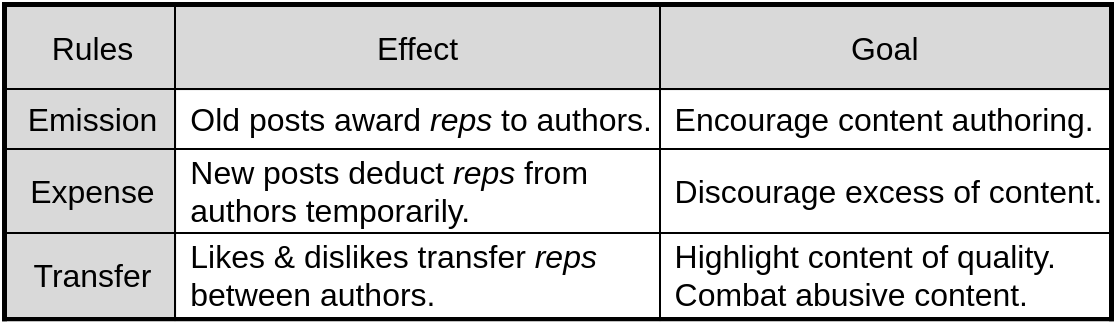
\includegraphics[width=0.6\textwidth]{general.png}
    \caption{General reputation rules in public chains.}
    \label{fig.general}
\end{wrapfigure}

Freechains~\cite{fcs.sbseg20} is a content dissemination P2P protocol in which
users post messages to a topic (or chain) and other users subscribed to the
same chain eventually receive the messages.
%
Each chain behaves as an independent blockchain with an innovative reputation
mechanism that moderates content through likes and dislikes and, at the same
time, guarantees consensus in the order of messages.
%
Figure~\ref{fig.general} summarizes the general reputation rules, in which
users can spend tokens named \emph{reps} to post and rate content in the
chains:
    a post initially penalizes authors until it consolidates and counts positively;
    a like is a positive feedback that helps subscribers to distinguish content amid excess;
    a dislike is a negative feedback that revokes content when crossing a threshold.

The reputation mechanism of Freechains works towards our goal of subjective
correctness in \AMT as follows:
    dislikes can revoke abusive and malicious posts, thus preserving integrity;
    likes can favor posts with more quality, thus preserving accuracy.

The basic command-line API of Freechains is as follows:

\begin{itemize}
\item \code{fc keys ...} \\
    Creates cryptographic keys as user identities.
\item \code{fc chains join ...} \\
    Joins a chain to post and read content.
\item \code{fc chain post ...} \\
    Posts a message to a chain.
\item \code{fc chain get ...} \\
    Reads a post from a chain.
\item \code{fc chain (like|dislike) ...} \\
    Likes or dislikes a post in the chain.
\item \code{fc chain consensus ...} \\
    Shows all posts from a chain in consensus order.
\item \code{fc peer sync ...} \\
    Synchronizes a chain with a remote peer.
\end{itemize}

Except for \code{fc~peer~sync}, none of the commands connect to the network,
but only modify the local replica.
%
Users need to call \code{fc~keys} only once to create a public-private key pair
as an identity to operate in the chains.
%
For each chain of interest, users need to call \code{fc~chains~join} with the
same arguments such that they are compatible when synchronizing.
%
Once a chain is created, users can call \code{fc~chain~get} and
\code{fc~chain~post} to read and write messages.
%
A chain can be traversed in total order through \code{fc~chain~consensus},
which enumerates all post ids, which can be read through \code{fc~chain~get}.
%
Finally, \code{fc~peer~sync} exchanges missing posts between replicas.

Regarding the integration with \AMT, we use \code{fc~chain~post/get} to persist
Automerge operations serialized through \code{AM.save} and \code{AM.load}.
We also rely on \code{fc~peer~sync} as a synchronization layer to Automerge,
which now ensures integrity and accuracy via \code{fc~chain~consensus}.

Like Automerge, Freechains is also designed for
\emph{local-first software}~\cite{p2p.local}, given that most commands only
modify the local replica.
For this reason, concurrent posts are not only encouraged, but are also
inevitable.
The next example simulates two users \code{A} and \code{B} posting concurrently
to chain \code{\#test}:

\noindent
{\footnotesize
\begin{minipage}[t]{0.5\textwidth}
\begin{verbatim}
// USER A
$ fc keys pubpvt "passwd-A"
<pub-A> <pvt-A>
$ fc chains join "#test" \
    <pub-A>=20 <pub-B>=10
$ fc chain "#test" post inline \
    "msg-A" --sign=<pvt-A>
$ fc peer <ip-B> sync "#test"
$ fc chain "#test" consensus
msg-A --> msg-B
\end{verbatim}
\end{minipage}
\begin{minipage}[t]{0.5\textwidth}
\begin{verbatim}
// USER B
$ fc keys pubpvt "passwd-B"
<pub-B> <pvt-B>
$ fc chains join "#test" \
    <pub-A>=20 <pub-B>=10
$ fc chain "#test" post inline \
    "msg-B" --sign=<pvt-B>
$ fc peer <ip-A> sync "#test"
$ fc chain "#test" consensus
msg-A --> msg-B
\end{verbatim}
\end{minipage}
}

\begin{wrapfigure}{R}{0.3\textwidth}
    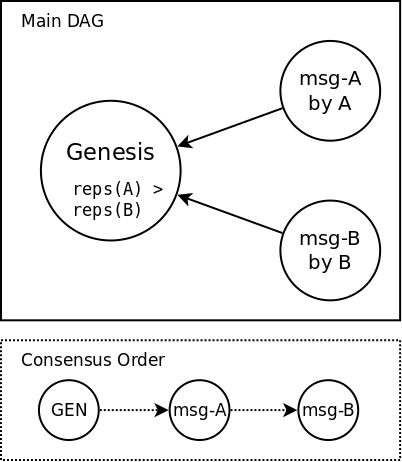
\includegraphics[width=0.3\textwidth]{dag.png}
    \caption{A chain DAG with corresponding consensus order.}
    \label{fig.dag}
\end{wrapfigure}

Users \code{A} and \code{B} first generate their identities and join the
public chain \code{\#test} with the same arguments.
The keys after \code{join~"\#test"} represent the pioneers, which share an
initial reputation to moderate the chain~\cite{fcs.sbseg20}.
In the example, we determine that user \code{A} has twice of \code{B}'s
reputation in order to illustrate the consensus mechanism of Freechains.
Then, the users call \code{chain~post} concurrently with distinct messages and
signatures, which creates a fork in the chain.
%
After the users synchronize with \code{peer~sync}, the posts are exchanged and
the chain reaches the state of Figure~\ref{fig.dag}.
The chain fork represented in the DAG suggests that only a partial order of
posts is possible.
Nevertheless, the call to \code{chain~consensus} is guaranteed to always
return the same order of posts \code{msg-A~-->~msg-B} in both sides.

The consensus algorithm of Freechains provides a total order of posts, even in
the presence of forks.
Freechains employs a topological sorting algorithm to favor reputation when
deciding between branches in a chain DAG~\cite{fcs.sbseg20}.
%
In Figure~\ref{fig.dag}, user \code{A} has more reputation in the common
prefix, therefore, the branch at the top must be ordered first.

\begin{comment}
The algorithm works as follows~\cite{fcs.sbseg20}:
\begin{itemize}
\item
    The common prefix is evaluated to extract the reputation of all users with
    posts.
    In Figure~\ref{fig.dag}, the common prefix only contains the genesis
    block, in which user \code{A} has more reputation than user \code{B}.
\item
    Each branch in the fork is evaluated to extract the set of users with
    posts.
    In Figure~\ref{fig.dag}, the branch at the top contains user \code{A} and
    the branch at the bottom contains user \code{B}.
\item
    The branches are ordered based on the sum of reputation of their users, but
    considering the common prefix.
    In Figure~\ref{fig.dag}, user \code{A} had more reputation in the common
    prefix, therefore, the branch at the top is ordered first.
\end{itemize}
\end{comment}

Even though Freechains provide means to preserve integrity and accuracy, it
does not support structured datasets with attached semantics, since it
represents content as a simple linked list of binary blobs stored in chains.

\section{AM-Tools}
\label{sec.amtools}

\AMT reconciles Automerge and Freechains to provide a solid foundation to
manipulate JSON datasets in permissionless networks, while preserving
consistency, integrity, and accuracy:
%
On the one hand, Automerge supports decentralized structured JSON datasets with
fine-grained merging policies, but which are still subject to integrity abuse
and corner-case inaccuracies.
%
On the other hand, Freechains resists malicious peers and guarantees a total
order of editions, but does not support datasets with automatic merges.

As described in the Introduction, \AMT is composed of 3 utility sets:
\amrw allows to read and write portions of JSON files.
\amdiff \& \ampatch obtain and apply differences between JSON files.
\amcheckout \& \amcommit persist JSON files to their corresponding blockchain.

\subsection{\amrw: JSON Command-Line Editor}

\amrw%
    %\footnote{\amrw: \url{https://github.com/fabiobosisio/amrw}}
    \footnote{\amrw: \url{https://github.com/<hidden-anonymous>}}
is a facade to hide the complexity of \code{AM.change}, and also provides a
uniform syntax to manipulate JSON files.
Recall from Section~\ref{sec.automerge} that, because CRDTs need track all
operations, JSON files cannot be edited directly.

The basic command-line API of \amrw is as follows:

\begin{itemize}
\item \code{AM-rw <file> init} \\
    Initializes a file as an empty JSON object (based on \code{AM.init}).
\item \code{AM-rw <file> <path>... (read | write <op>)} \\
    Reads a value from or writes to a JSON file (based on \code{AM.change}).
    A \code{<path>...} is a sequence of field or index accesses to navigate the
    JSON.
    A \code{write <op>} can insert, set, or remove a field or index in the
    JSON.
\end{itemize}

The next example writes to a JSON to reach the final state {list: ['A','B']}:

{\footnotesize
\begin{verbatim}
$ AM-rw "test.am" init
$ AM-rw "test.am" write object ins "list" array
$ AM-rw "test.am" field "list" write array ins 0 string "A"
$ AM-rw "test.am" field "list" write array ins 1 string "B"
$ AM-rw "test.am" read
{ list: [ 'A', 'B' ] }
\end{verbatim}
}

In the first write, we use an empty path, which navigates to the root object,
in which we add a field \code{list} as an empty array.
The writes in sequence navigate to the array field \code{list}, and insert
strings \code{'A'} and \code{'B'}.

Even though \amrw is more verbose in comparison to Automerge's
\code{AM.change}, it provides a uniform syntax to manipulate JSON files.
In addition, as a command-line tool, it can be used from outside JavaScript
even by non programmers.

\subsection{\amdiff \& \ampatch}

\amdiff \& \ampatch%
    %\footnote{\ampatch: \url{https://github.com/fabiobosisio/ampatch}}
    \footnote{\amdiff \& \ampatch: \url{https://github.com/<hidden-anonymous>}}
are counterparts to textual \emph{diff \& patch} UNIX tools, but which work on
Automerge's JSON internal format.

The basic command-line API of \amdiff \& \ampatch is as follows:

\begin{itemize}
\item \code{AM-diff <old> <new>} \\
    Calculates the differences between the given files.
\item \code{AM-patch <cur> <patch>} \\
    Applies the patch to the given file.
\end{itemize}

The next example illustrates how to extract the differences between an old and
a new file, and then recreate the new file by applying the obtained difference
into the old file:

{\footnotesize
\begin{verbatim}
$ AM-diff  "old.am" "new.am" > "old-new.diff"
$ AM-patch "old.am" "old-new.diff" > "rec.am"
\end{verbatim}
}

At the end, \code{new.am} and \code{rec.am} are guaranteed to be equal files.

Just like standard version control systems, the idea is that storing
\emph{diffs} to recreate the full history of a given file history is more
efficient than storing all individual versions of that file.
%
With \AMT, we rely on Freechains to store these \emph{diffs}, which users can
rate and possibly revoke, affecting the consensus order that recreates the file
history.

\subsection{\amcheckout \& \amcommit}

The final piece of \AMT is to synchronize JSON \emph{diffs} between replicas
and then update local versions of files based on the global consensus.

\amcheckout \& \amcommit%
    %\footnote{\amcheckout \& \amcommit: \url{https://github.com/fabiobosisio/ampatch}}
    \footnote{\amcheckout \& \amcommit: \url{https://github.com/<hidden-anonymous>}}
are counterparts to standard \emph{checkout \& commit} VCS tools, but which use
Freechains for persistence, conflict resolution, and synchronization.

The basic command-line API of \amcheckout \& \amcommit is as follows:

\begin{itemize}
\item \code{AM-checkout <chain>} \\
    Recreates the JSON file from the chain.
\item \code{AM-commit <chain> --sign=<pvt>} \\
    Posts the file differences into the chain with the author signature.
\end{itemize}

The next example illustrates how to checkout a JSON file, modify it, and then
commit it back into the chain:

{\footnotesize
\begin{verbatim}
$ AM-checkout "test"
$ AM-rw "test.am" field "list" write array ins 2 string "C"
$ AM-commit "test" --sign=<pvt>
\end{verbatim}
}

The synchronization between replicas must be done in pairs through
\code{fc~peer~sync}, as described in Section~\ref{sec.freechains}.
%
The command \amcheckout traverses the chain replica \code{test}, starting from
its genesis block holding the initial JSON, and then calling \ampatch, in
consensus order, for each block holding the \emph{diffs}.
The result is the local file \code{test.am} with the most recent JSON.
%
The command \amrw makes local modifications to \code{test.am}, but which do not
affect the chain replica \code{test}.
%
Finally, the command \amcommit compares the local file with the chain replica
file calling \amdiff, and then posts the \emph{diffs} back into the chain.

Commits must be signed because of the reputation system of Freechains, which
preserves the repository integrity and accuracy.
For instance, commits from authors with no reputation, such as Sybils trying to
SPAM the repository are rejected by default, since they require welcoming likes
from existing users in the chain~\cite{fcs.sbseg20}.
Likewise, malicious commits from existing users can be revoked a posteriori
with dislikes from other users with more reputation.

\begin{wrapfigure}{R}{0.6\textwidth}
    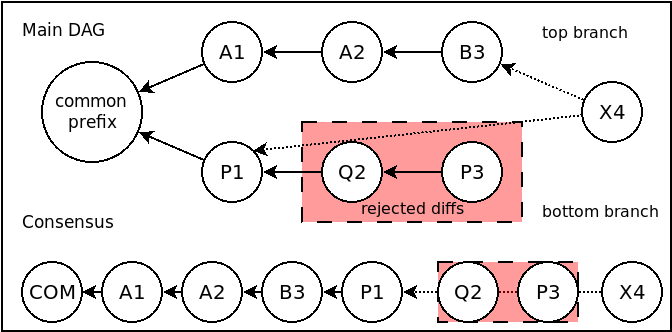
\includegraphics[width=0.6\textwidth]{conflicts.png}
    \caption{Conflict resolution in \AMT.}
    \label{fig.conflicts}
\end{wrapfigure}

As discussed in Section~\ref{sec.automerge}, not all complications in
repositories are due to Sybils or malicious editions:
\AMT inherits the local-first nature of Automerge and Freechains in which
with irreconcilable conflicts are inevitable.
%
Therefore, our main contribution with \AMT is on how to merge conflicting
branches automatically to reach a final version that reflects the intent of the
majority of the network.

Figure~\ref{fig.conflicts} illustrates a legitimate scenario that cannot
preserve the intent of both branches at the same time.
Each node in the main DAG is a \emph{diff} holding a JSON edition (e.g.,
\code{A1} and \code{Q2}).
\AMT recreates the file by applying the \emph{diffs} in consensus order.
Based on the common prefix, the consensus guarantees that all patches in the
top branch applies successfully, thus satisfying the intent of the majority of
the network.
Nevertheless, as a best effort policy, the \emph{diffs} in the bottom branch,
are also applied in sequence, but may or may not succeed.
In the example, there is a merge conflict only when trying to apply \code{Q2},
which is identified by \amcheckout based on \ampatch through
\code{AM.getConflicts}.
%
In such situations, \amcheckout ignores all remaining \emph{diffs} because they
can no longer reach a consistent state without human intervention.
In addition, \amcommit ensures that further \emph{diffs} such as \code{X4} are
linked back only to succeeded patches (i.e., \code{B3} and \code{P1}),
effectively merging the branches and ensuring that the file remains in a
consistent state automatically.

In summary, \AMT reconciles Automerge and Freechains to provide a decentralized
version control system with automatic merges that preserves consistency,
integrity, and accuracy, even in the presence of Sybils and malicious users.

\begin{comment}
\subsection{Putting It All Together}

We now illustrate how to combine Freechains and \AMT to XXX:

{\footnotesize
\begin{verbatim}
$ fc keys pubpvt "my-passwd"                                    : 01
<pub> <pvt>                                                     : 02
$ fc chains join "#test" <pub>                                  : 03
$ AM-rw "test.am" init                                          : 04
$ AM-rw "test.am" write object ins "title" string "Test File"   : 05
$ AM-commit "#test" --sign=<pvt>                                : 06
$ fc peer <ip> sync '#test'                                     : 07
$ AM-checkout "#test" --sign=<pvt>                              : 08
$ AM-rw "test.am" read                                          : 09
{title: 'Test File', date: 'July 2023'}                         : 10
\end{verbatim}
}
\end{comment}

\bibliographystyle{abbrv}
\bibliography{amtools}

\end{document}
